\documentclass[12pt]{article}
\usepackage{graphicx} %handles figures
\usepackage{anysize} %handles margins
\usepackage{amsfonts}
\usepackage{bm}
\usepackage{framed}
\usepackage[utf8]{inputenc}
\usepackage[english]{babel}
\usepackage{natbib}
\usepackage{url}
\usepackage{amsmath}
\DeclareMathOperator{\sgn}{sgn}
\usepackage{mathrsfs}
\usepackage{amssymb}
\usepackage{subcaption}
\usepackage{fancyhdr}
\usepackage{float}
\usepackage{amsfonts}
\usepackage{geometry}
\usepackage{caption}
\usepackage{listings}
\usepackage{array}
\usepackage{breqn}
\usepackage{indentfirst}
\usepackage{multirow}
\usepackage{physics}
\usepackage{minted}


% for formatting pseudocode
\usepackage{algorithm}
\usepackage[noend]{algpseudocode}
\usepackage[colorlinks,linkcolor=blue]{hyperref}
\makeatletter
\def\BState{\State\hskip-\ALG@thistlm}
\makeatother
% header and footed
\usepackage{fancyhdr}
\usepackage{lastpage}
\pagestyle{fancy}
%\chead{\bfseries  Team No. 212}
\rhead{Page \thepage\ of \pageref{LastPage}}
\cfoot{}
\lstset{
  basicstyle=\ttfamily,
  columns=fullflexible,
  frame=single,
  breaklines=true,
}

\begin{document}

\thispagestyle{empty}

\begin{center}
{\bf\large{Team No. 212}}

\vspace{1em}

{\large{Problem B}}


\vspace{4em}
{\Large{Quadcopter Stability in Wind}}
\end{center}

\vspace{5em}

\begin{abstract}
In this article, we estimate the maximum windspeed that allows the quadcopter to stay within 20cm from the target. We use python to build a physical simulation system, a thrust control system that can control the quadcopter to react to the wind and maintain its stability and a wind simulator . By inputting  two basic patterns of wind(periodic and noise) into our simulation with different magnitude, we get the average time that the quadcopter is able to stay within range. We find that periodic wind poses greater threats to safety operation than the dominant wind with noise.

\textbf{Keywords}: Quadcopter dynamics, Linear Control, Newton-Euler method, Controller design, Wind simulation, Stability analysis


\end{abstract}
\newpage

\tableofcontents
\newpage

\section{Introduction}
Quadcopter unmanned aerial vehicles (UAVs) are used widely both in industry and in academic research nowadays. Some applications with precise operation requires high stability of the platform.

Wind is the major disturbance source effecting the stability of the UAVs. The real wind usually has time-dependent magnitude and direction, which can easily threaten the safety of the equipment. Thus the maximum wind speed that allows safe operation is an important parameter to estimate the UAV performance.

In this article, we are going to develop a simulation method to determine the maximum wind speed that can allow the drone to stay within $20$ cm of the target. 

%Sketch the method you are going to use. 
%Give an overview (one sentence) of the structure of your paper.
In Model section, the physics simulation system is first proposed, which models the dynamic of the drone given the wind. Then is the thrust controller, which generates the best response given the wind and the drone's current info. Finally, the wind simulator is  proposed, which can both generate periodic or noised wind. 

% To present the results of the simulation method, we also developed a simple flight control system and connect it with the simulation program. In real applications, the simulation can be applied to some more advanced control system and test the performance of the quadcopter. 

In Results section, we will first give the brief summary of our model's simulation result and give the maximum wind speed that allows safe operation. Then, the detailed data will be given with clear image illustration to validate our statement.

Finally,we will draw conclusions and discuss the advantages and  and advantages of our model and give comments on how to improve the model.
 



% Roller coaster is one of the most exciting recreation facilities in amusement park. In this article, we are going to design a roller coaster which is safe and exciting. We will first give a concept diagram of our roller coaster’s whole trajectory, then divide it into five parts and analyse them respectively. We are going to use the basic kinematics laws to construct second order ODEs for the motion of the roller coaster car, and apply the Euler Method to obtain an approximate solution for the ODEs, from which we could obtain the velocity and acceleration at any instant of time.
% In Model Section, we will first give our method of judgement of safety and excitement, then introduce the basic laws and methods we will use in this project. Moreover, for each part of our trajectory, we will give a simple model with parameters.
% In Result Section, we will first give the overall results of our whole model, and give the proof of the safety and excitement. Then we will explain in details about how we obtain the results and the motion of the car in each part of the trajectory.
% Finally we will draw a conclusion and discuss the limitations and advantages of our model and give some suggestions about how to improve the model.


\section{Model}
\subsection{Problem Overview} In this article, we are going to estimate the maximum windspeed that allows the quadcopter to stay within 20cm from the target. We will first simplify the quadcopter dynamics model to reduce the calculation complexity in algorithm. Based on the rigid body dynamics, we then derive equations of motions and then use python to build a physical simulation system for the quadcopter. We then develop a thrust control system that can control the quadcopter to react to the wind and maintain its stability. By inputting basically two patterns of wind(periodic and noise) into our simulation with different magnitude, we run the simulation repeatly and get the average time that the quadcopter is able to stay within desired range. If the time is large enough, the corresponding windspeed is allowed for the safe operation. The maximum windspeed can be found accordingly.

\begin{figure}[htbp]
\centering
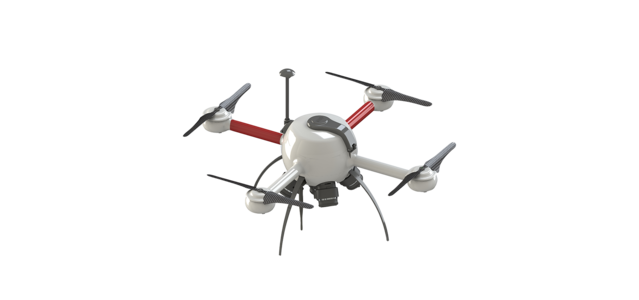
\includegraphics[width= 0.7\linewidth, angle =0]{Images/quadcopter.png}
\caption{Quadcopter overview.}
\label{fig:1}
\end{figure}

\subsection{Assumption and Definition}
\subsubsection{Quadcopter model simplification}
The drone we used in our model has a total mass of $1.5 $kg, and is powered by four rotors which can each generate a thrust up to $7$ N.

The major mass of the quadcopter is concentrated on the platform in the middle. Therefore, in order to simplify the dynamics equation of motion during the operation of the quadcopter, we assume that the platform in the center is a homogeneous sphere with a radius $r=10cm$ and a mass $m=1kg$. Four rotors are arranged in a square, each with a mass $m_{r}=0.125kg$, and a distance of $d = 50cm$ from the sphere center. We assume that the four rods connecting the rotor to the central sphere are light enough that it can be ignored in the dynamics model. The model frame is showed in Figure \ref{fig:model}.

As for staying within 20 cm, as our model, including the thrust control system algorithm, is rough, if the quadcopter is able to stay within 20 cm around the target for 30 s, it is believed that if the optimized control algorithm is given, the quadcopter can stay for as long as possible. Thus, the objective of the simulation is to find the maximum wind speed that the quadcopter can resist to stay within 20 cm around the target for 30 s.

\subsubsection{Aerodynamics of the model}
According to the study on the propeller aerodynamics \cite{bib1}, the aerodynamic effects applied to the rotor are evaluated by integrating, along each rotor blade, the aerodynamic force per surface increment.

By integrating the lift per surface increment, we obtain the lift force LF (or thrust)
\begin{equation}
 \mathbf{F_{L}}=\rho c R^{3} \omega^{2} C_{L \alpha}\left(\frac{\alpha_{0}}{3}-\frac{\bar{w}+L\left(\varepsilon_{1} q-\varepsilon_{2} p\right)}{2 R|\omega|}\right) \hat{\mathbf{z}_{\mathbf{B}}}
\end{equation}
where $R$ is the radius of the rotor blade, $\rho$ is the air density, $U$ is the airspeed, $c$ is the blade width, $C_{L \alpha}$ is the lift coefficient, $\alpha_{0}$ its pitch angle at rest. The coefficients $\varepsilon_{1}$ and $\varepsilon_{2}$ depend on the rotor under consideration.

The first item with $\omega^{2}$ is far more larger than other items. Thus, the equation for the lift force can be safely reduced to \begin{equation}
\mathbf{F_{L}}=\frac{1}{3}\rho c R^{3} \omega^{2} C_{L \alpha}\alpha_{0} \hat{\mathbf{z}_{\mathbf{B}}}
\end{equation}

Here the lift coefficient $C_{L\alpha}$ can be approximate by the average pitch angle $\overline{\alpha}$ \cite{bib3} of the blade. \begin{equation}
    C_{L\alpha}=c_{l}sin(\overline{\alpha})cos(\overline{\alpha}).
\end{equation}

In our model, we set $\rho=1.225kg/m^{3}$, $c=3cm$, $R=5cm$, $\overline{\alpha}=0.78$, thus $$\mathbf{F_{L}}=0.01\omega^{2}$$.

For the drag force on the rotors, we neglect the interactions of the vehicle dynamics onto the aerodynamics effects, thus the drag force caused by the rotors is zero.

For the drag force on the middle sphere 
\begin{equation}
\label{sphereDrag}
\mathbf{F_{d}}=\frac{1}{2}\rho A \norm{\boldsymbol{u_r}} \boldsymbol{u_r} C_{d},
\end{equation}where $A=\pi r^{2}$ is the cross section area of the sphere, $\boldsymbol{u_r}=\boldsymbol{w}-\dot{\boldsymbol{\xi}}$ is the velocity of wind relative to the quadcopter in the ground frame and $C_{d}$ is the drag coefficient. Here we set $C_{d}=1.$

\subsection{Physics simulation system}

\begin{figure}[htbp]
\centering
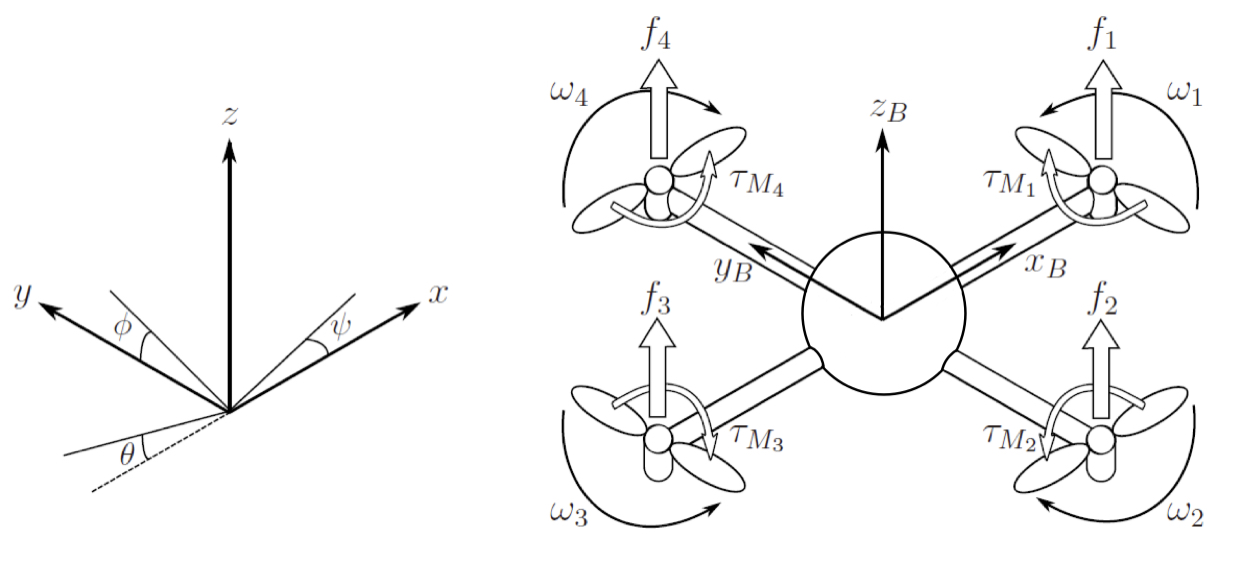
\includegraphics[width= 0.7\linewidth, angle =0]{Images/Model.png}
\caption{The simplified frame for a quadcopter.}
\label{fig:model}
\end{figure}
The dynamics of the quadcopter's motion is approached with rigid body mechanics in \cite{bib2}. We adopted notations from the paper but also made necessary simplifications to the model. The quadcopter has 6 degrees of freedom, 3 for translational motion and 3 for rotation.
Both the ground frame and the body frame are considered for solving the motion of the quadcopter. The axes of the body frame $x_B, y_B$ and $z_B$ are indicated in Figure\ref{fig:model}. The origin of the body frame is located at the center of mass of the quadcopter, which is the center of the central sphere in our model.

In the ground frame, the Cartesian coordinates $\mathrm{x}, \mathrm{y}, \mathrm{z}$ is denoted by $\boldsymbol{\xi}$. The posture of the quadcopter is described with Euler angle $\boldsymbol{\eta}$ with components $\phi, \theta$ and $\psi$, as shown in Figure\ref{fig:model}.

$$
\boldsymbol{\xi}=\left[\begin{array}{l}
x \\
y \\
z
\end{array}\right], \quad \boldsymbol{\eta}=\left[\begin{array}{l}
\phi \\
\theta \\
\psi
\end{array}\right]
$$
In the body frame, we denote the linear velocity with $\boldsymbol{V}_{B}$ and the angular velocities with $\boldsymbol{\nu}$.
$$
\boldsymbol{V}_{B}=\left[\begin{array}{l}
v_{x, B} \\
v_{y, B} \\
v_{z, B}
\end{array}\right], \quad \boldsymbol{\nu}=\left[\begin{array}{l}
p \\
q \\
r
\end{array}\right]
$$
The rotation matrix from the body frame to the inertial frame is an orthogonal matrix
$$
\boldsymbol{R}=\left[\begin{array}{ccc}
C_{\psi} C_{\theta} & C_{\psi} S_{\theta} S_{\phi}-S_{\psi} C_{\phi} & C_{\psi} S_{\theta} C_{\phi}+S_{\psi} S_{\phi} \\
S_{\psi} C_{\theta} & S_{\psi} S_{\theta} S_{\phi}+C_{\psi} C_{\phi} & S_{\psi} S_{\theta} C_{\phi}-C_{\psi} S_{\phi} \\
-S_{\theta} & C_{\theta} S_{\phi} & C_{\theta} C_{\phi}
\end{array}\right]
$$

The transformation matrix for angular velocities from the inertial frame to the body frame is $\boldsymbol{W}_{\eta},$ and from the body frame to the inertial frame is $\boldsymbol{W}_{\eta}^{-1},$ as shown in

\begin{equation}
\dot{\boldsymbol{\eta}}=\boldsymbol{W}_{\eta}^{-1} \boldsymbol{\nu}, \quad\left[\begin{array}{c}
\dot{\phi} \\
\dot{\theta} \\
\dot{\psi}
\end{array}\right]=\left[\begin{array}{ccc}
1 & S_{\phi} T_{\theta} & C_{\phi} T_{\theta} \\
0 & C_{\phi} & -S_{\phi} \\
0 & S_{\phi} / C_{\theta} & C_{\phi} / C_{\theta}
\end{array}\right]\left[\begin{array}{l}
p \\
q \\
r
\end{array}\right]
\end{equation}


\begin{equation}
\boldsymbol{\nu}=\boldsymbol{W}_{\eta} \dot{\boldsymbol{\eta}}, \quad\left[\begin{array}{c}
p \\
q \\
r
\end{array}\right]=\left[\begin{array}{ccc}
1 & 0 & -S_{\theta} \\
0 & C_{\phi} & C_{\theta} S_{\phi} \\
0 & -S_{\phi} & C_{\theta} C_{\phi}
\end{array}\right]\left[\begin{array}{c}
\dot{\phi} \\
\dot{\theta} \\
\dot{\psi}
\end{array}\right]
\end{equation}

in which $T_{x}=\tan (x)$. The matrix $\boldsymbol{W}_{\eta}$ is invertible if $\theta \neq (2 k-1) \phi / 2$, $k \in \mathbf{Z}$

In our simplified model of the quadcopter, the inertia of its body (excluding the rotors) can be obtained as the inertia of tensor of a sphere:
\begin{equation}
\boldsymbol{I} = \frac{1}{5}mr^2 \boldsymbol{I}_3
\end{equation}

The angular velocities the four rotors are denoted by $\omega_i$ ($i = 1, 2, 3, 4$). For simplicity the air drag arising from the rotation and angular acceleration of the rotors are omitted.

We use $T$ to denote the combined force given by the rotors in the $z_B$ direction. In the body frame, the combined force is
\begin{equation}
\boldsymbol{T}_{B}=\left[\begin{array}{l}
0 \\
0 \\
T
\end{array}\right]
\quad \text{where} \quad
T=\sum_{i=1}^{4} f_{i}=k \sum_{i=1}^{4} \omega_{i}^{2}
\end{equation}

Also, the torque caused by the thrust is
\begin{equation}
\boldsymbol{\tau}_{B}=\left[\begin{array}{c}
\tau_{\phi} \\
\tau_{\theta} \\
\tau_{\psi}
\end{array}\right]=\left[\begin{array}{c}
d(f_4 - f_2) \\
d(f_3 - f_1) \\
0
\end{array}\right]
\end{equation}
The physical significance of the torque is clear: by altering the difference between $f_4$ and $f_2$, rolling movement can be obtained; by altering the difference between $f_3$ and $f_1$, one can obtain pitch movement.
The acquirement of yaw movement is a little more subtle, and we'll soon notice that yaw movement arises from gyroscopic force $\Gamma$ in Newton-Euler equations.

The translational and rotational motion of the quadcopter can be fully described with Newton-Euler equations. For translational motion, it's easier to use the ground frame: 

\begin{equation}
\label{translationEquation}
m \ddot{\boldsymbol{\xi}}=\boldsymbol{G}+\boldsymbol{R} \boldsymbol{T}_{B} + \boldsymbol{F}_{\text{wind}}
\end{equation}

\begin{equation}
\left[\begin{array}{c}
\ddot{x} \\
\ddot{y} \\
\ddot{z}
\end{array}\right]=-g\left[\begin{array}{c}
0 \\
0 \\
1
\end{array}\right]+\frac{T}{m}\left[\begin{array}{c}
C_{\psi} S_{\theta} C_{\phi}+S_{\psi} S_{\phi} \\
S_{\psi} S_{\theta} C_{\phi}-C_{\psi} S_{\phi} \\
C_{\theta} C_{\phi}
\end{array}\right]
\end{equation}
where $F_{\text{wind}}$ is the drag force given in Equation\ref{sphereDrag}.
For rotational movement, we can obtain the angular acceleration with

\begin{equation}
\boldsymbol{I} \dot{\boldsymbol{\nu}}+\boldsymbol{\nu} \times(\boldsymbol{I} \boldsymbol{\nu})+\boldsymbol{\Gamma}=\boldsymbol{\tau}
\end{equation}

\begin{equation}
\label{angularEquation}
\dot{\boldsymbol{\nu}}=\boldsymbol{I}^{-1}\left(-\left[\begin{array}{c}
p \\
q \\
r
\end{array}\right] \times\left[\begin{array}{c}
I_{x x} p \\
I_{y y} q \\
I_{z z} r
\end{array}\right]-I_{r}\left[\begin{array}{c}
p \\
q \\
r
\end{array}\right] \times\left[\begin{array}{l}
0 \\
0 \\
1
\end{array}\right] \omega_{\Gamma}+\boldsymbol{\tau}\right)
\end{equation}

where $\omega_{\Gamma}=\omega_{1}-\omega_{2}+\omega_{3}-\omega_{4}$ and $I_r$ is the moment of inertia of each rotor relative to its axis of symmetry. 

With the angular acceleration in body frame obtained, we can derive that in the ground frame with $\boldsymbol{W}_{\eta}$:

\begin{equation}
\label{groundAngularAcceleration}
\begin{aligned}
\ddot{\boldsymbol{\eta}} &=\frac{\mathrm{d}}{\mathrm{d} t}\left(\boldsymbol{W}_{\eta}^{-1} \boldsymbol{\nu}\right)=\frac{\mathrm{d}}{\mathrm{d} t}\left(\boldsymbol{W}_{\eta}^{-1}\right) \boldsymbol{\nu}+\boldsymbol{W}_{\eta}^{-1} \dot{\boldsymbol{\nu}} \\
&=\left[\begin{array}{ccc}
0 & \dot{\phi} C_{\phi} T_{\theta}+\dot{\theta} S_{\phi} / C_{\theta}^{2} & -\dot{\phi} S_{\phi} C_{\theta}+\dot{\theta} C_{\phi} / C_{\theta}^{2} \\
0 & -\dot{\phi} S_{\phi} & -\dot{\phi} C_{\phi} \\
0 & \dot{\phi} C_{\phi} / C_{\theta}+\dot{\phi} S_{\phi} T_{\theta} / C_{\theta} & -\dot{\phi} S_{\phi} / C_{\theta}+\dot{\theta} C_{\phi} T_{\theta} / C_{\theta}
\end{array}\right] \boldsymbol{\nu}+\boldsymbol{W}_{\eta}^{-1} \dot{\boldsymbol{\nu}}
\end{aligned}
\end{equation}

\subsection{Thrust control system}
\label{Sec:Flight control}
Our thrust control system is designed as an linear optimization problem for $f_1, f_2, f_3, f_4$. In each step, our goal is to
\begin{itemize}
    \item maximize the component of the velocity in the direction that points to the origin.
    \item maximize the component of angular acceleration in the direction opposite to the current angular velocity.
\end{itemize}

In other words, our goal is to
    \begin{equation}
        \text{maximize  } (\dot{\boldsymbol{\xi}} + \boldsymbol{\xi} \Delta t) \cdot (- \boldsymbol{r}) \text{  subject to  } f_i \leq 7 \text{N } (i= 1, 2, 3, 4)
    \end{equation}
    and 
    \begin{equation}
        \text{maximize  } (\boldsymbol{\dot{\boldsymbol{\eta}}} + \ddot{\boldsymbol{\eta}} \Delta t) \cdot (- \boldsymbol{\eta})
        \text {  subject to } f_i \leq 7 \text{N } (i = 1, 2, 3, 4)
    \end{equation}
    
    with Equation\ref{translationEquation}, Equation\ref{angularEquation} and Equation\ref{groundAngularAcceleration} these two optimization goals can be reduced to
    \begin{equation}
        \text{minimize } (\boldsymbol{R} \boldsymbol{T}^{B}) \cdot \boldsymbol{\xi} 
    \end{equation}
    and
    \begin{equation}
        \text{minimize } (\boldsymbol{W}_{\eta}^{-1} \boldsymbol{I}^{-1} \boldsymbol{\tau}) \cdot \boldsymbol{\eta}
    \end{equation}
    The gyroscopic forces $\bm{\Gamma}$ can introduce non-linear terms of the thrust forces, but they are neglected because of their small magnitude compared with $\bm{\tau}$.
    

    Finally our problem has the form of minimizing $\sigma (f_1 + f_2 + f_3 + f_4)$ and minimizing $w_1 (f_4 - f_2) + w_2 (f_3 - f_1)$

    where
    \begin{equation}
        \sigma = \boldsymbol{R}\left[\begin{array}{c}
0 \\
0 \\
1
\end{array}\right] 
\cdot \boldsymbol{\xi},
    \end{equation}
    
    \begin{equation}
        w_1 = \boldsymbol{W}_{\eta}^{-1} \boldsymbol{I}^{-1}\left[\begin{array}{c}
1 \\
0 \\
0
\end{array}\right]\cdot \boldsymbol{\eta},
    \end{equation}
    and
    \begin{equation}
        w_2 = \boldsymbol{W}_{\eta}^{-1} \boldsymbol{I}^{-1}\left[\begin{array}{c}
0 \\
1 \\
0
\end{array}\right]\cdot \boldsymbol{\eta},
    \end{equation}

As a linear optimization problem, 
The pseudocode for controlling is given in Algorithm\ref{ThrustControlAlgorithm}, where $\epsilon, \delta$ and $\zeta$ are parameters for controlling each adjustment.
\begin{algorithm}
\caption{Thrust Control algorithm}
\label{ThrustControlAlgorithm}
\begin{algorithmic}[1]
\Procedure{Update Thrust Control}{}
\State $f_1 \gets f_1 - \sgn(\sigma) \epsilon$
\State $f_2 \gets f_2 - \sgn(\sigma) \epsilon$
\State $f_3 \gets f_3 - \sgn(\sigma) \epsilon$
\State $f_4 \gets f_4 - \sgn(\sigma) \epsilon$
\State $f_4 \gets f_4 - \sgn(w_1) \delta$
\State $f_2 \gets f_2 + \sgn(w_1) \delta$
\State $f_3 \gets f_3 - \sgn(w_2) \zeta$
\State $f_1 \gets f_1 + \sgn(w_2) \zeta$
\EndProcedure
\end{algorithmic}
\end{algorithm}

\subsection{Wind pattern}
Real wind conditions are usually not steady, characterized by constant changes in direction and magnitude. 
The main characteristics of wind speed are randomness, intermittentness and sudden change. Therefore, when simulating the wind field, we decompose the wind speed vector into dominant wind $ \boldsymbol{w}_d $, periodic wind $ \boldsymbol{w}_p $, and random wind $ \boldsymbol{w}_r $.

\subsubsection{Dominant wind}
Since wind is relatively continuous to time in most cases, we define a dominant wind speed vector $\boldsymbol{w}_r  $ within the time range of our simulation test as a constant vector. For convenience, we set it along the x axis.\begin{equation}
    \boldsymbol{w}_d=k \hat{i}. 
\end{equation}

\subsubsection{Periodic wind}
In order to better simulate the dynamic changes of real wind, we introduce a periodically changing wind based on the dominant wind, which is specifically expressed as a sinusoidal wind speed vector with initial phase superimposed on the dominant wind in three directions.
\begin{equation}
        \left\{\begin{array}{c} 
            \begin{aligned}   
            &w_{px}=u \left(t-t_{bx}\right)W_{x}sin\left(2\pi\left(\frac{t-t_{bx}}{T_{px}}\right)\right),\\
            &w_{py}=u \left(t-t_{by}\right)W_{y}sin\left(2\pi\left(\frac{t-t_{by}}{T_{py}}\right)\right),\\
            &w_{pz}=u \left(t-t_{bz}\right)W_{z}sin\left(2\pi\left(\frac{t-t_{bz}}{T_{pz}}\right)\right).
            \end{aligned}
            \end{array}
            \right.
\end{equation}
Here $ u(t-t_{bi})$ is the step function that switches from $ 0 $ to $ 1 $ when $ t=t_{bi} $, $ \boldsymbol{T}_{pi} $ is the period of the periodic wind from the $ i $th coordinate and $t_{bi} $ is the begin time of the sinusoidal wind from $ i $th coordinate.


\subsubsection{Random noise}
Considering different disturbance in the open environment, the random wind component $ \overrightarrow{\bm{w_{r}}} $ is also added into windspeed vector. The random wind here is simulated by adding a noise into the dominant wind. The added random noise follows the Gaussian distribution with the probability density \begin{equation}
    p(x)=\frac{1}{\sqrt{2 \pi \sigma^{2}}} e^{-\frac{(x-\mu)^{2}}{2 \sigma^{2}}}
\end{equation}
where $\mu$ is the mean and $\sigma$ the standard deviation. 
The function has its peak at the mean, and its ``spread" increases with the standard deviation. This implies that the noise added into the dominant wind is more likely to return to the mean value, rather than those far away. For each step of time, the wind vector is incremented by the noise \begin{equation}\label{it}
    \left\{\begin{array}{c}
        \begin{aligned}
            &w_{rx}(t+\Delta t)=w_{rx}+\Delta w_{rx,n},\\
            &w_{ry}(t+\Delta t)=w_{ry}+\Delta w_{ry,n},\\
            &w_{ry}(t+\Delta t)=w_{rz}+\Delta w_{rz,n}.
        \end{aligned}
    \end{array}
    \right.
\end{equation}
Here $ \boldsymbol{w}_{r, i}$ is the random wind component along the $ i $th coordinate, $ \Delta \boldsymbol{w}_{ri,n} $ is the increment following the Guassian normal distribution added to the $ i $ th random wind component each step of time in the iteration.

However, because the noise we introduced is the vector sum of three one-dimensional random walk along $ x,y,z $ coordinate, the random windspeed will gradually drifting from its mean magnitude $0$. To avoid the noise to change the magnitude of the dominant windspeed, a correction item in direct proportion to the current random windspeed is introduced into the iteration. Thus, Eq.(\ref{it}) can be refined to \begin{equation}
\left\{\begin{array}{c}
        \begin{aligned}
            &w_{rx}(t+\Delta t)=w_{rx}+\Delta w_{rx,n}-C_{I}w_{rx},\\
            &w_{ry}(t+\Delta t)=w_{ry}+\Delta w_{ry,n}-C_{I}w_{ry},\\
            &w_{ry}(t+\Delta t)=w_{rz}+\Delta w_{rz,n}-C_{I}w_{rz}.
        \end{aligned}
    \end{array}
    \right.
\end{equation}
Here $C_{I}$ is the coeffient introduced to eliminate the drift. The detail method is introduced in section \ref{Sec:Flight control}.

Combining the dominant, periodic and random windspeed, the real wind condition can be approached, In our physics simulation, the windspeed input will be chosen from the vector sum of these components 
\begin{equation}
\boldsymbol{w} = \boldsymbol{w}_d+ \boldsymbol{w}_p + \boldsymbol{w}_r.
\end{equation}



%\begin{figure}[htbp]
%\centering
%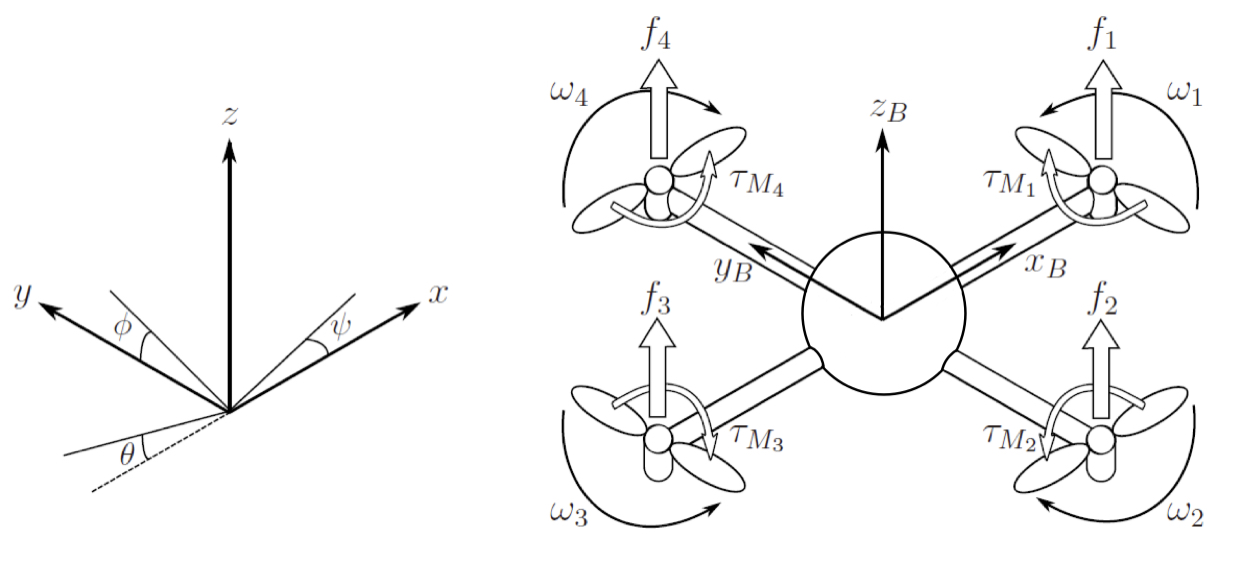
\includegraphics[width= 0.7\linewidth, angle %=0]{Images/Model.png}
%\caption{The simplified frame for a quadcopter.}
%\label{fig:1}
% %\end{figure}

% ...
% \begin{itemize}

% \item  Formulate the problem (do not simply copy the problem description).
% \item  Include any references to this problem (or a very similar one) you may have found in the literature (acknowledge any references!, see 5.). Here are examples of references \cite{kittel05}. For details please see the attached \LaTeX file \cite{ashcroft02}.
% \item Highlight the laws of physics behind the problem;
% \item Argue for the approach you will be using;
% Formulation of the model: here you should clearly formulate all assumptions, hypotheses and introduced variables.  You should also point out why you choose this model.
% \item You may include a sketch/figure/graph if it is necessary to explain your model.

% \end{itemize}

\section{Results}
\subsection{Dominant wind with random noise}
In order to find the maximum wind speed that complies with our definition of the problem in Section2.2.1, wind patterns with different speed distributions were tested in our simulation environment. We aim to find the maximum wind speed that enables the quadcopter to stay around the target within 20 cm for 30 s. For this reason, the simulation for each wind model is suspended once the distance from the origin reaches 20cm. $t_20$ for each wind model is obtained as the average of 10 simulations under the same condition. The simulation data is summarized in Table\ref{tab: sim}.

Referring from the table, we can roughly find the maximum wind speed $v_M = 5$ m/s.

 \begin{table}[H] 
 \centering 
 \begin{tabular}{|c|c|c|}
 \hline
 Wind Speed [m/s]& Deviation of the Wind Speed [m/s]&  $t_{20}$ [s] \\ \hline \hline
   2  & 0.01  & 45.55 \\ \hline
 2  & 0.11  & 36.59\\ \hline
 2  & 0.21 & 28.27\\ \hline
 2  & 0.31  & 23.58\\ \hline
 2  & 0.41  & 22.11 \\ \hline
 2  & 0.51  & 18.79\\ \hline
 2  & 0.61  & 12.10\\ \hline
 3  & 0.01  & 48.70\\ \hline
 3  & 0.11  & 35.68\\ \hline
 3  & 0.21  & 31.36\\ \hline
 3  & 0.31  & 15.73\\ \hline
 3  & 0.41  & 17.83\\ \hline
 3  & 0.51  & 15.02\\ \hline
 3  & 0.61  & 12.75\\ \hline
 4  & 0.01  & 53.68\\ \hline
 4  & 0.11  & 45.48\\ \hline
 4  & 0.21  & 30.09\\ \hline
 4  & 0.31  & 20.69\\ \hline
 4  & 0.41 & 16.35\\ \hline
 4  & 0.51  & 14.25\\ \hline
 4  & 0.61  & 12.85\\ \hline
 5  & 0.01  & 54.13\\ \hline
 5  & 0.11  & 54.89\\ \hline
 5  & 0.21  & 45.45\\ \hline
 5  & 0.31  & 15.63\\ \hline
 5  & 0.41 & 23.66\\ \hline
 5  & 0.51  & 13.81\\ \hline
 5  & 0.61  & 10.56\\ \hline
 6  & 0.01  & 60.59\\ \hline
 6  & 0.11  & 53.93\\ \hline
 6  & 0.21  & 26.38\\ \hline
 6  & 0.31  & 21.37\\ \hline
 6  & 0.41 & 19.43\\ \hline
 6  & 0.51  & 10.83\\ \hline
 6  & 0.61  & 8.41\\ \hline
 7  & 0.01  & 42.67\\ \hline
 7  & 0.11  & 28.90\\ \hline
 7  & 0.21  & 34.13\\ \hline
 7  & 0.31  & 21.08\\ \hline
 7  & 0.41  & 20.81\\ \hline
 7  & 0.51  & 13.50\\ \hline
 7  & 0.61  & 9.95\\ \hline
 \end{tabular}% 
 \caption{Simulation Data} 
 \label{tab: sim}% 
 \end{table}% 
To make our simulation more convincing, four sample simulation trajectories are plotted in Figure \ref{fig: traj}. Each subfigure was simulated under wind speed of 5 m/s and deviation of 0.1m/s. The trajectories consist of positions of center of mass during the simulations. These plots demonstrate how the control system manages to keep the quadcopter near the origin when it's subject to the wind. 

The wind field is also visualized in Figure \ref{fig: wind} to give an clear intuition of how it varies in direction and magnitude through time. The dataset of wind speed in the figure has deviation of 0.2 m/s. Each line represents the wind speed at an instant. The color of the end point of the lines vary continuously from deep brown to pale yellow.

\begin{figure}[H]
\begin{subfigure}{.5\textwidth}
\centering
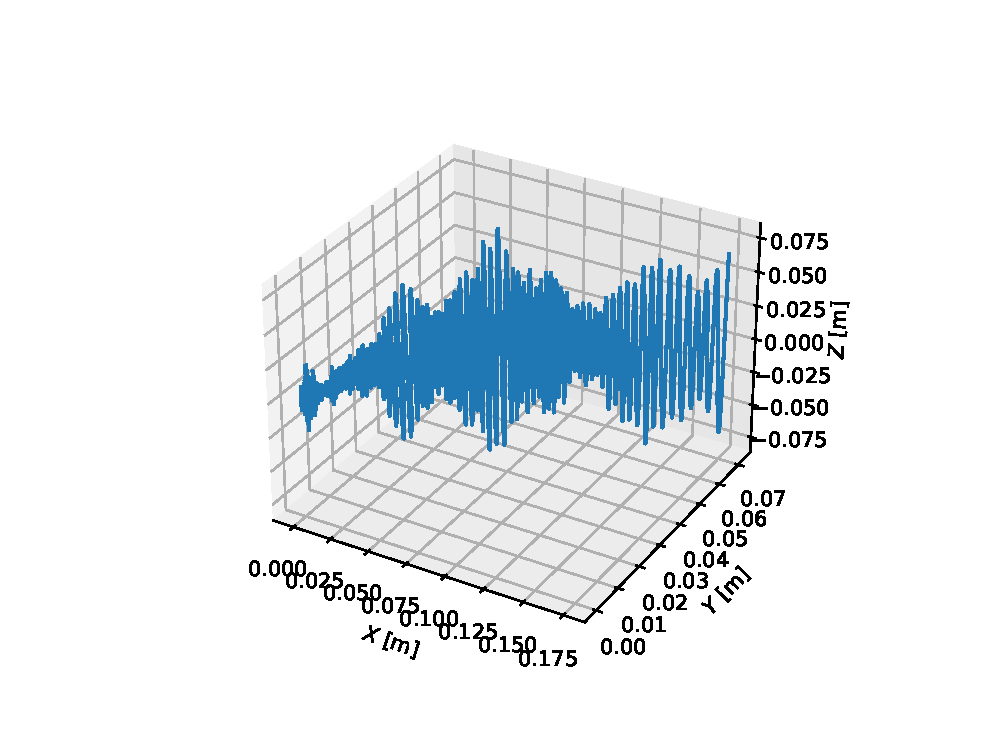
\includegraphics[width=\linewidth]{Images/trajectory 1.eps}
\caption{Trajectory 1}
\end{subfigure}
\hfill
\begin{subfigure}{.5\textwidth}
\centering
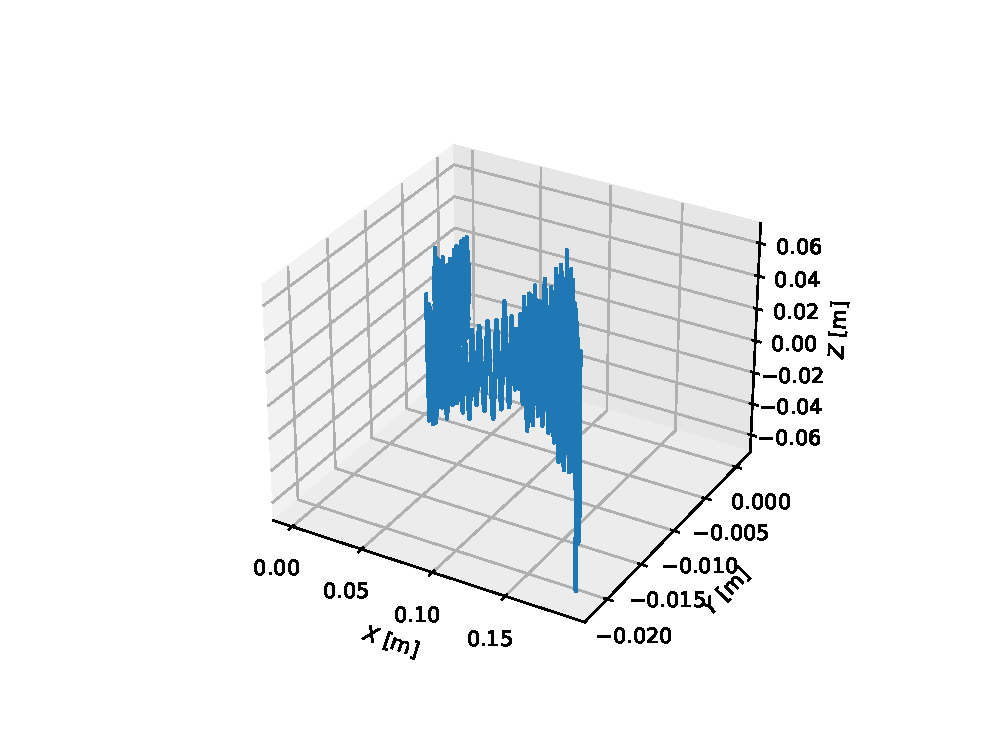
\includegraphics[width=\linewidth]{Images/trajectory 2.eps}
\caption{Trajectory 2}
\end{subfigure}
\hfill
\begin{subfigure}{.5\textwidth}
\centering
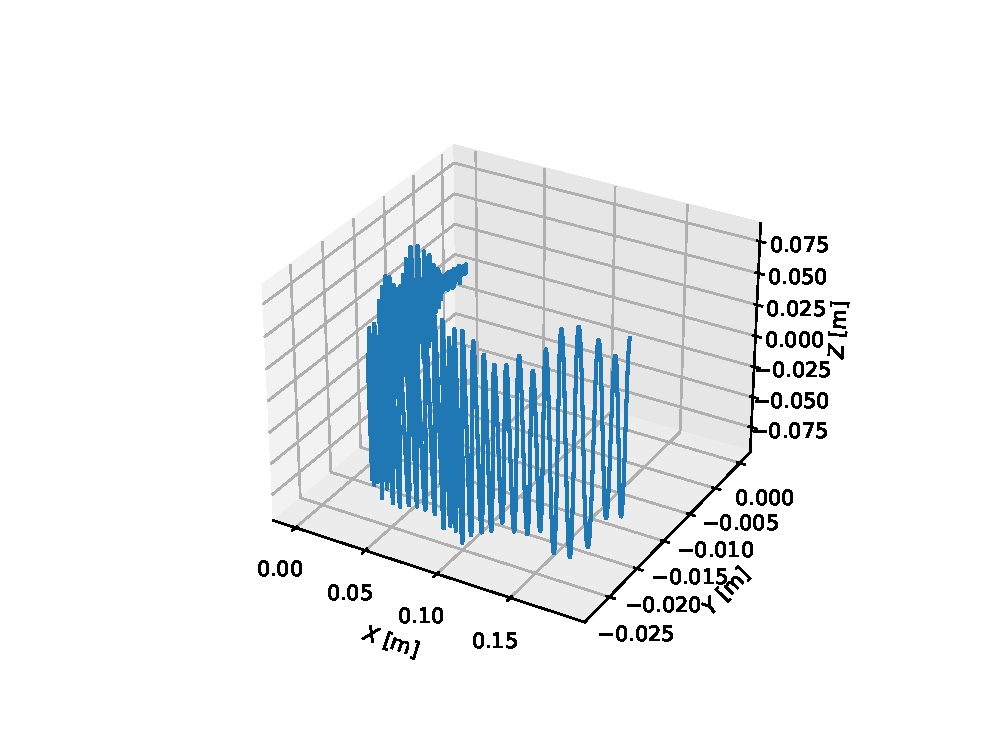
\includegraphics[width=\linewidth]{Images/trajectory 3.eps}
\caption{Trajectory 3}
\end{subfigure}
\begin{subfigure}{.5\textwidth}
\centering

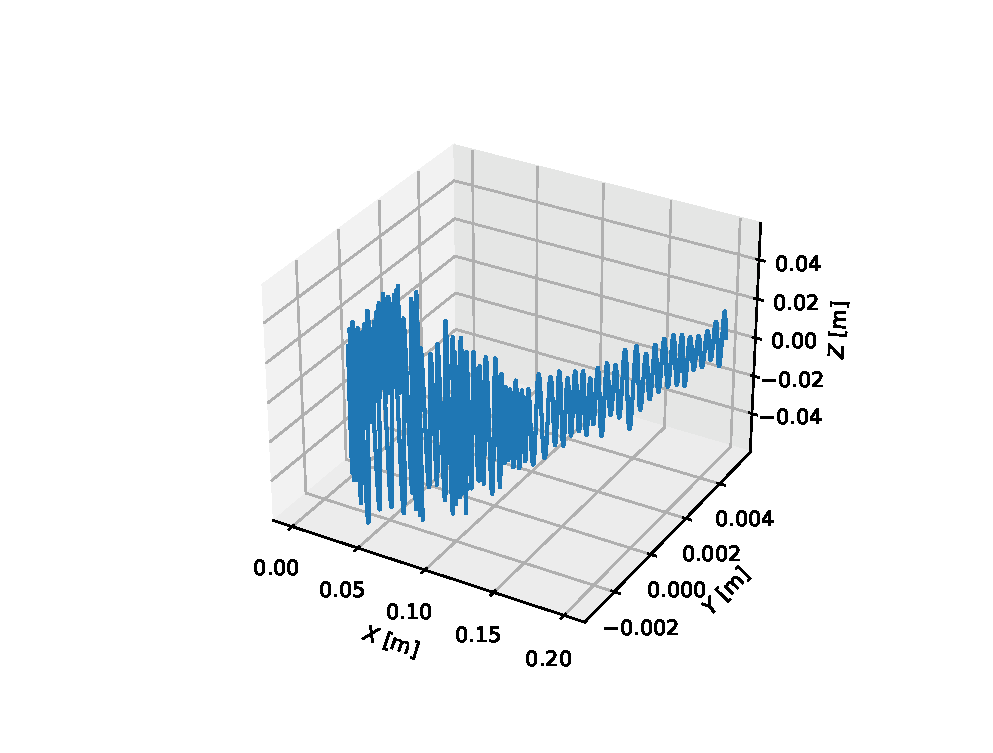
\includegraphics[width=\linewidth]{Images/trajectory 4.eps}
\caption{Trajectory 4}
\end{subfigure}
\caption{Sample Trajectories for Wind Speed = 5 m/s}
\label{fig: traj}
\end{figure}

\begin{figure}[H]
    \centering
    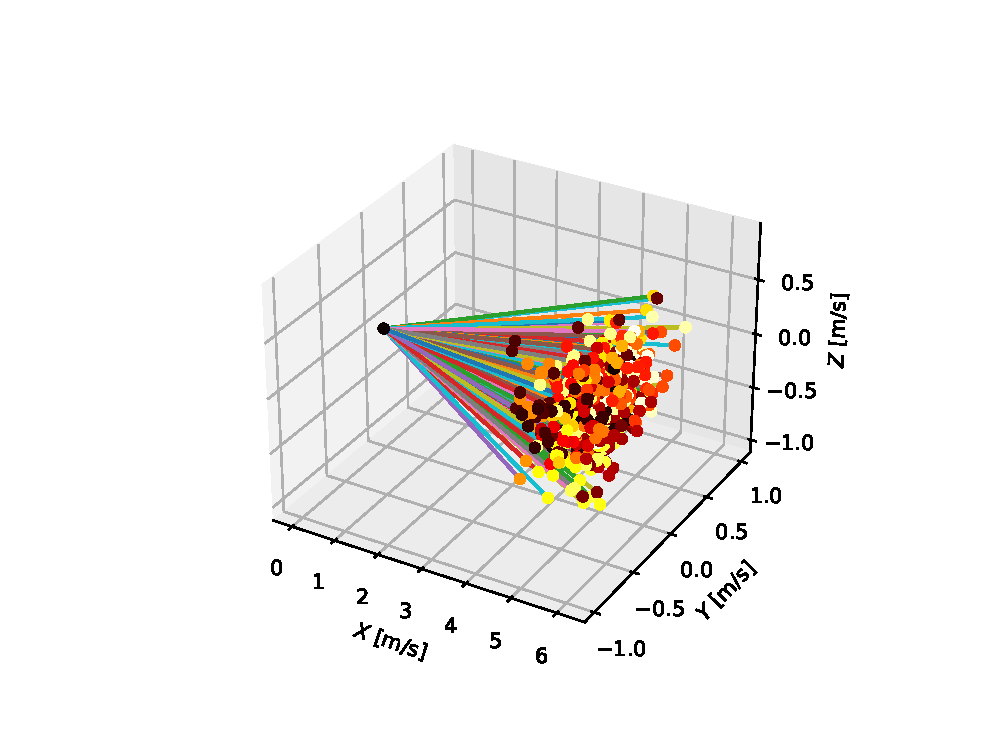
\includegraphics[width=.8\linewidth]{Images/wind.eps}
    \caption{Visualization of Wind}
    \label{fig: wind}
\end{figure}



\subsection{Periodic wind}
From Fourier analysis we know that any periodical wind can be decomposed into a series of wind with sinusoidal velocity components. Figure \ref{fig: windSin} exhibits the possible wind speed with sinusoidal velocity components.

Therefore the study of periodical wind with sinusoidal velocity components is crucial as it can help us predicate the behavior of the quadcopter under more general periodical wind patterns.
In this section we observe periodic wind with sinusoidal velocity component in the x-axis direction.
In order to find the maximum wind speed that complies with our definition of the problem in Section2.2.1, wind with different amplitude and frequency were tested in our simulation environment. Again, $t_20$ denotes the time at which the distance from the origin reaches 20cm. The simulation data is summarized in Table\ref{tab: simSin} and Table\ref{tab:simSin2}.

Referring from the table, we can conclude that our control model cannot handle wind with varying magnitude as perfectly as it does with dominant wind patterns. With fixed amplitude, the stability becomes worse at the frequency of the change of wind's velocity increases. However, we can also notice that the stability is less sensitive to increasement of frequency at lower amplitudes.

Under frequency $f = 0.01$ Hz, the performance reaches our expectation only when the amplitude of the velocity of wind is no larger than $0.95$ m/s. When the frequency becomes larger, the quadcopter will be able to keep itself stable under lower amplitudes.

For periodic wind, four sample simulation trajectories are plotted in Figure \ref{fig: trajSin}. Each subfigure was simulated under amplitude $1.2$m and frequency $0.01$ Hz. The trajectories consist of positions of center of mass during the simulations. These plots demonstrate how the control system manages to keep the quadcopter near the origin when it's subject to periodical wind.



\begin{figure}[H]
\begin{subfigure}{.5\textwidth}
\centering
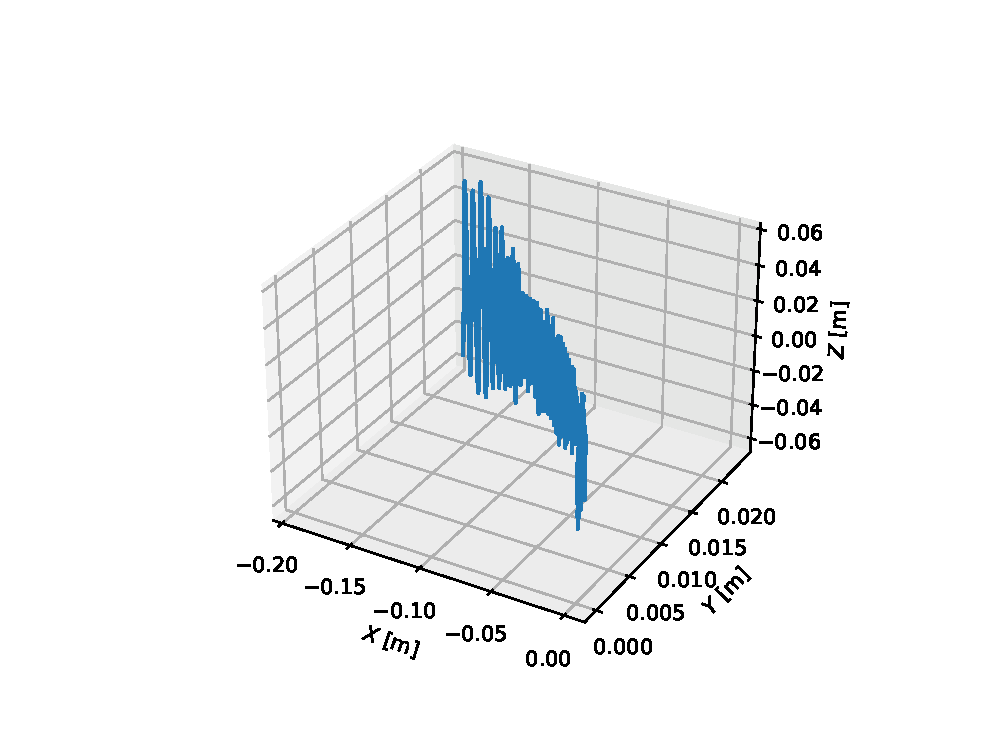
\includegraphics[width=\linewidth]{Images/trajectory_sin.eps}
\caption{Trajectory 1}
\end{subfigure}
\hfill
\begin{subfigure}{.5\textwidth}
\centering
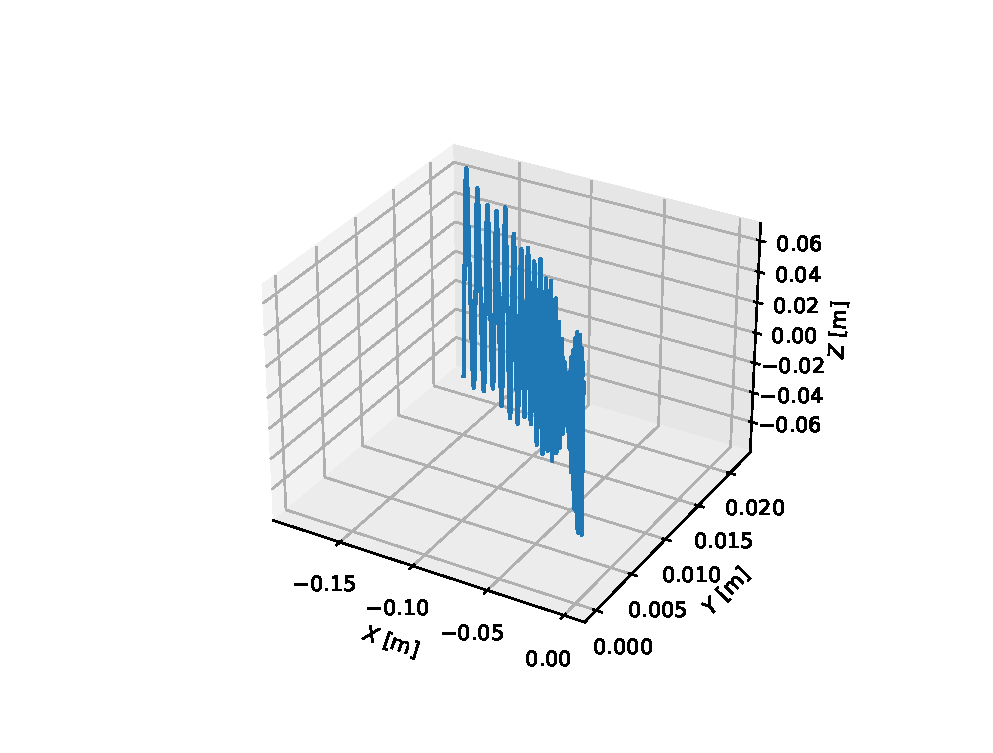
\includegraphics[width=\linewidth]{Images/trajectory_sin copy.eps}
\caption{Trajectory 2}
\end{subfigure}
\hfill
\begin{subfigure}{.5\textwidth}
\centering
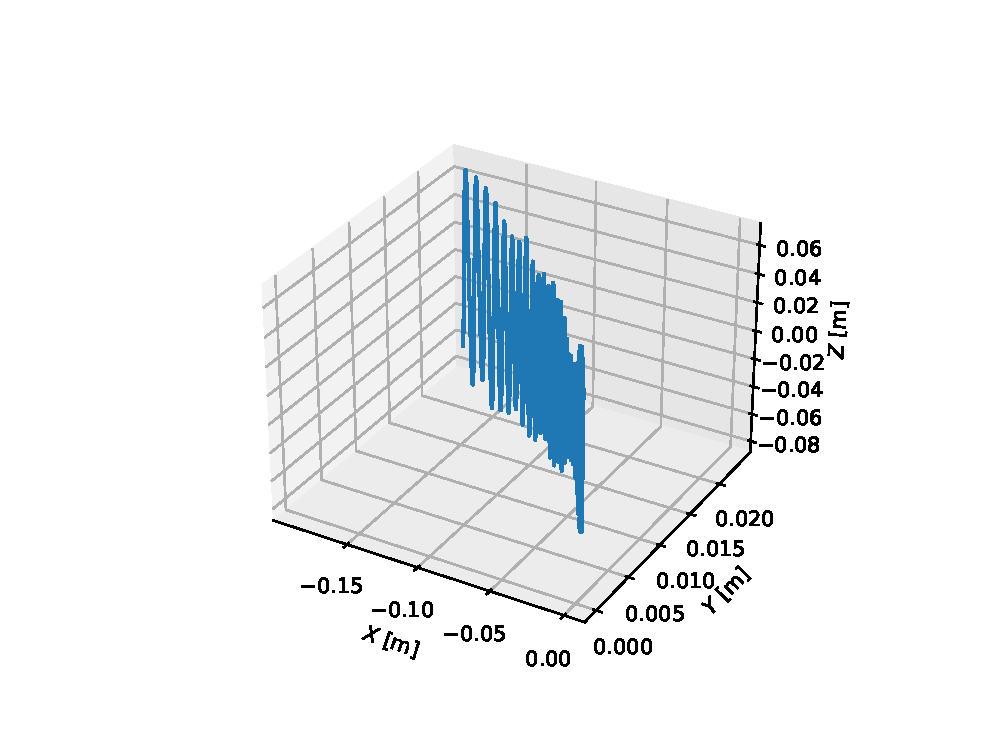
\includegraphics[width=\linewidth]{Images/trajectory_sin copy 2.eps}
\caption{Trajectory 3}
\end{subfigure}
\begin{subfigure}{.5\textwidth}
\centering

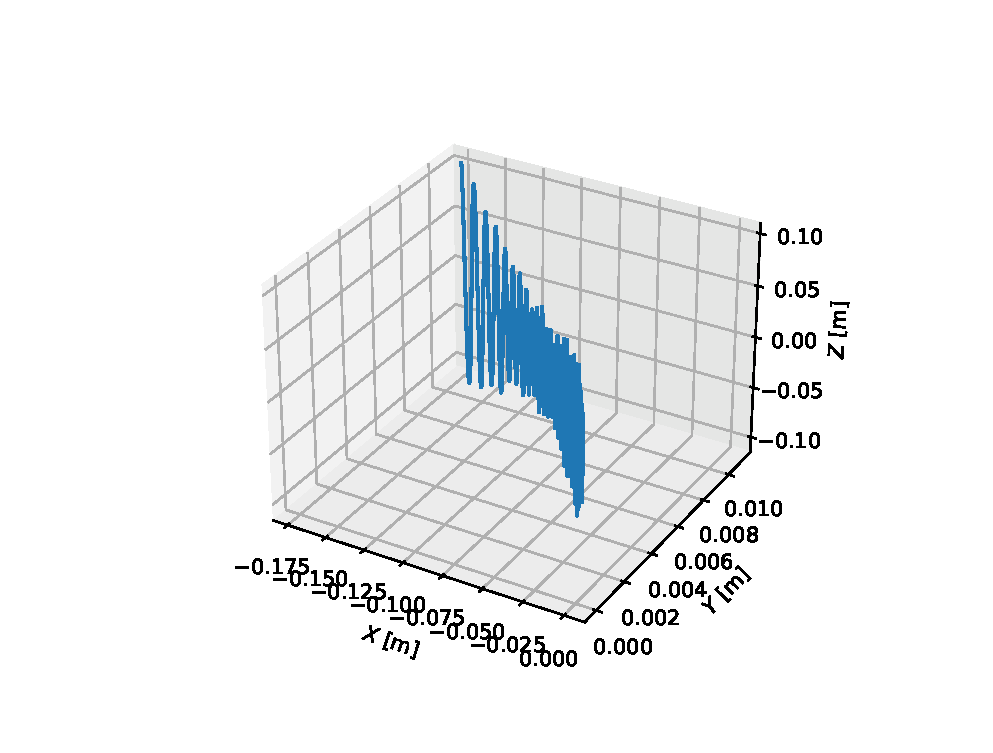
\includegraphics[width=\linewidth]{Images/trajectory_sin copy 3.eps}
\caption{Trajectory 4}
\end{subfigure}
\caption{Sample Trajectories for Wind Speed = 5 m/s}
\label{fig: trajSin}
\end{figure}

\begin{figure}[H]
    \centering
    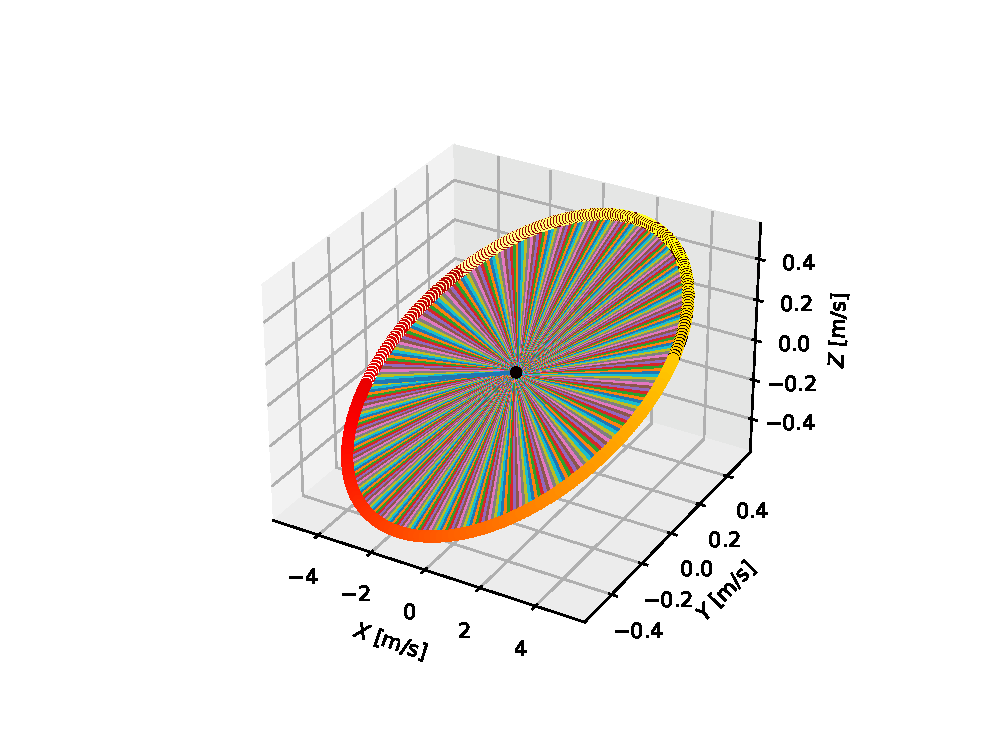
\includegraphics[width=.8\linewidth]{Images/wind_sin.eps}
    \caption{Visualization of Wind}
    \label{fig: windSin}
\end{figure}




 \begin{table}[H] 
 \centering 
 \begin{tabular}{|c|c|c|}
 \hline
 Speed Amplitude [m/s] & frequency [Hz] & $t_{20}$ [s] \\ \hline


1.001 & 0.01 & 26.54 \\ \hline
1.001 & 0.02 & 20.50 \\ \hline
1.001 & 0.03 & 18.08 \\ \hline
1.001 & 0.04 & 16.60\\ \hline
1.001 & 0.05 & 15.78 \\ \hline
1.001 & 0.060 & 15.28 \\ \hline
1.001 & 0.070 & 15.27 \\ \hline
2.001 & 0.01 & 17.73 \\ \hline
2.001 & 0.02 & 13.45 \\ \hline
2.001 & 0.03 & 11.63 \\ \hline
2.001 & 0.04 & 10.53 \\ \hline
2.001 & 0.05 & 9.72 \\ \hline
2.001 & 0.060 & 9.12 \\ \hline
2.001 & 0.070 & 8.66 \\ \hline
3.001 & 0.01 & 14.66 \\ \hline
3.001 & 0.02 & 10.67 \\ \hline
3.001 & 0.03 & 8.99 \\ \hline
3.001 & 0.04 & 8.070\\ \hline
3.001 & 0.05 & 7.47 \\ \hline
3.001 & 0.060 & 7.00 \\ \hline
3.001 & 0.070 & 6.630\\ \hline



 \end{tabular}% 
 \caption{Periodic Wind Simulation Data Table 1} 
 \label{tab: simSin}% 
 \end{table}% 

 \begin{table}[H] 
 \centering 
 \begin{tabular}{|c|c|c|}
 \hline
 Speed Amplitude [m/s] & frequency [Hz] & $t_{20} [s]$ \\ \hline

 0.7 & 0.001 & 44.86 \\ \hline
0.7 & 0.011 & 32.46 \\ \hline
0.7 & 0.021 & 24.67 \\ \hline
0.7 & 0.031 & 21.93 \\ \hline
0.7 & 0.041 & 21.05 \\ \hline
0.7 & 0.051 & 21.05 \\ \hline
0.7 & 0.061 & 21.31 \\ \hline
0.75 & 0.001 & 44.58 \\ \hline
0.75 & 0.011 & 30.70 \\ \hline
0.75 & 0.021 & 24.09 \\ \hline
0.75 & 0.031 & 21.29 \\ \hline
0.75 & 0.041 & 20.19 \\ \hline
0.75 & 0.051 & 19.96 \\ \hline
0.75 & 0.061 & 20.20 \\ \hline
0.8 & 0.001 & 44.26 \\ \hline
0.8 & 0.011 & 30.09 \\ \hline
0.8 & 0.021 & 23.26 \\ \hline
0.8 & 0.031 & 20.24 \\ \hline
0.8 & 0.041 & 19.24 \\ \hline
0.8 & 0.051 & 18.76 \\ \hline
0.8 & 0.061 & 19.01 \\ \hline
0.85 & 0.001 & 47.57 \\ \hline
0.85 & 0.011 & 27.78 \\ \hline
0.85 & 0.021 & 21.95 \\ \hline
0.85 & 0.031 & 19.73 \\ \hline
0.85 & 0.041 & 18.33 \\ \hline
0.85 & 0.051 & 17.88 \\ \hline
0.85 & 0.061 & 17.89 \\ \hline
0.9 & 0.001 & 45.60 \\ \hline
0.9 & 0.011 & 27.46 \\ \hline
0.9 & 0.021 & 21.31 \\ \hline
0.9 & 0.031 & 19.03 \\ \hline
0.9 & 0.041 & 17.83 \\ \hline
0.9 & 0.051 & 17.12 \\ \hline
0.9 & 0.061 & 17.08 \\ \hline
0.95 & 0.001 & 47.43 \\ \hline
0.95 & 0.011 & 26.25 \\ \hline
0.95 & 0.021 & 20.77 \\ \hline
0.95 & 0.031 & 18.52 \\ \hline
0.95 & 0.041 & 17.11 \\ \hline
0.95 & 0.051 & 16.38 \\ \hline
0.95 & 0.061 & 16.00 \\ \hline



 \end{tabular}% 
 \caption{Periodic Wind Simulation Data Table 2} 
 \label{tab:simSin2}% 
 \end{table}% 








% \begin{itemize}

% \item Present the solution following from the model you have constructed.
% \item List ALL values of the numerical parameters you have used (you may do it in the caption of graphs/tables);
% \item All graphs, tables etc. appear in this part. They are used to illustrate how results depend on any parameters/initial conditions in the problem.  They should be clearly labeled.

% \item The error analysis is required if you report an experiment, also a numerical one. In our case it probably will not be needed.


% \begin{figure}[h]
% \begin{center}
% %\includegraphics[scale=0.5]{hm6_bar.eps}
% \caption{Put the figure's caption here. Give the values of all parameters ($a=1\ {\rm{m}}$, $C = 10^{-5}\ {\rm{kg}})$.  You may also do it directly in the graph.}
% \end{center}
% \end{figure}

% \item  Discuss the dependence of the results on the values of parameters. Highlight the trends, point out any unusual behavior/properties your model may display;


% \end{itemize}


\section{Discussion}
\subsection{Conclusion}
In this paper, we proposed a physics simulation system to simulate
\begin{itemize}
    \item the dynamics of the quadcopter;
    \item a thrust control system which controls the thrusts of the quadcopter, keeping the quadcopter near the origin;
    \item a wind simulator to simulate winds that vary in time and magnitude through time.
\end{itemize}

These three parts are combined to find the maximum wind speed, which is
\begin{itemize}
    \item for dominant wind with noise,
    \item for periodic wind.
\end{itemize}

We find that the maximum windspeed allowed for the quadcopter to stay within the desired range for at least $30s$ when the dominant wind with noise was applied is $5m/s$.

For the periodic wind pattern, our control model cannot handle wind with varying magnitude as perfectly as it does with dominant wind patterns. With fixed amplitude, the stability becomes worse at the frequency of the change of wind's velocity increases. 

Under frequency $f = 0.01$ Hz, the performance reaches our expectation only when the amplitude of the velocity of wind is no larger than $0.95 m/s$.

We can accordingly conclude that periodic wind poses greater threats to safety operation than the dominant wind with noise. 

\subsection{Advantages}
Though it's a simplified model, our simulation has many advantages.
\begin{enumerate}
    \item The physics simulation system is accurate.
    
    As the rigid body dynamics theorem is used comprehensively, our physics simulation system will have the exact behavior as the according simplified model in reality.
    \item The thrust control algorithm is original and has strong physics interpretation.
    
    The thrust control algorithm was derived purely by solving the Newton-Euler equations and extracting terms with linear dependence on the thrust from the  accelerations (both translational and angular). Thus, compared to the standard PID control algorithm \cite{bib4}, it does not only have far more less parameters to adjust, but also a much clearer connection to the model it controls.
    % TODO: ref a PID paper
    
    \item The wind simulator simulates different types of winds and is adjustable.
    
    Through the simulation mathematical models of the three parts of wind speed that compose the wind field, dominant wind, periodic wind and random wind are used to simulate the change process of wind speed over a period of time, so that the randomness, intermittentness and the mutant characteristics of the real wind field under external interference can be considered. 
    
\end{enumerate}

\subsection{Limitation and possible refinement}
    Due to time limit, our model still has some limitations that need further refinement.
\begin{enumerate}
    \item The shape of the quadcopter.
    
    In this article, we simplify the major part of the quadcopter as a sphere and omit the structure connecting the rotors and the middle platform. However, actually the moment of inertia of the rod structures also matters in the equations of rigid body dynamics. However, in our model, due to the symmetry, this additional item can be replaced by changing the mass distribution of our model and will not effect the final results.
    
    \item The omitted Gyro force 
    
    In our thrust control system, we neglect the Gyro force when the angular speed is changing according to time. However, the neglect is reasonable because the magnitude of the force is 1-2 order smaller than other force, e.g. lift force or drag force acting on the middle sphere. Also, this force is considered in our physics simulation to accurately predict the motion of the quadcopter.
    
    \item Air drag
    To reduce the complexity of calculation, we omitted the drag force acting on four rotors. According to the study on the aerodynamics of the propellers\cite{bib1}, the drag force mainly depends on the translational velocity of the quadcopter and the angular speed of pitch, roll and yaw. The simulation can be improved by adding these items into our functions of force in the programs.
    
\end{enumerate}



\begin{thebibliography}{99}
\bibitem{bib1}P. Bristeau, P. Martin, E. Salaün and N. Petit, ``The role of propeller aerodynamics in the model of a quadrotor UAV," 2009 European Control Conference (ECC), Budapest, 2009, pp. 683-688, doi: 10.23919/ECC.2009.7074482.

\bibitem{bib2}Luukkonen, Teppo. "Modelling and control of quadcopter." Independent research project in applied mathematics, Espoo 22 (2011).


\bibitem{bib3}R. Gill and R. D'Andrea, "Propeller thrust and drag in forward flight," 2017 IEEE Conference on Control Technology and Applications (CCTA), Mauna Lani, HI, 2017, pp. 73-79, doi: 10.1109/CCTA.2017.8062443.

\bibitem{bib4}J. Li and Y. Li, "Dynamic analysis and PID control for a quadrotor," 2011 IEEE International Conference on Mechatronics and Automation, Beijing, 2011, pp. 573-578, doi: 10.1109/ICMA.2011.5985724.
% \bibitem{ashcroft02} N.W. Ashcroft, N.D. Mermin, \textit{Solid state physics}, 2nd edition, Holt Rinehart \&
% Winston (2002), pages 101--103
\end{thebibliography}

\newpage
\appendix
\section{Source Code}

\begin{framed}
\lstinputlisting[language=Python, caption= Source Code]{sim.py}
\end{framed}
\end{document}